
\documentclass[answers, 12pt]{exam}
\usepackage{amsmath}
\usepackage{amsthm}
\usepackage{amsfonts}
\usepackage{amssymb}
\usepackage{mathrsfs}
\usepackage[brazil]{babel}
\usepackage[utf8]{inputenc}

\renewcommand{\qedsymbol}{$\blacksquare$}
\renewcommand{\thequestion}{\arabic{section}.\arabic{question}}
\renewcommand{\solutiontitle}{\noindent\textbf{Solução:}\enspace}

\footer{}{\thepage}{}

\title{	%EA044 - Planejamento e Análise\\ de Sistemas de Produção - 2S 2018\\
		% {\large \textit{Docente}: Matheus Souza}\\[2mm]
		{\Large Soluções para problemas selecionados da apostila\\[-0mm]
        \textit{Otimização Matemática e Pesquisa Operacional}\\[-2mm]
        de André R. Fioravanti e Matheus Souza}\\[2mm]
        -- Capítulo 2 --
}
\author{Plínio Santini Dester (\url{p103806@dac.unicamp.br})}

\begin{document}

%% Content goes here
\maketitle

*Em caso de dúvidas, sugestões ou correções, não hesite em mandar um e-mail.

\setcounter{section}{1}
\section{Problemas}

\begin{questions}

% 2.1  % % % % % % % % % % % % % % % % % % % % %
% \setcounter{question}{0}
\question{Considere os números reais $a_1 \le a_2 \le \dots \le a_n$. Encontre a solução dos seguintes problemas:
\begin{parts}
	\part $\min\sum_{i=1}^n|x-a_i|$;
    \part $\min\max\{|x-a_i|,i=1,\dots,n\}$;
    \part $\min\sum_{i=1}^n(x-a_i)^2$;
    \part $\max\prod_{i=1}^n|x-a_i|$.
\end{parts}
}
\begin{solution}
\begin{parts}
	\part Para o problema
    \[\min_{x\in\R}\sum_{i=1}^n|x-a_i|,\]
    note que a função objetivo não pertence à classe $\mathscr{C}^1$, logo não vale a condição necessária que a derivada precisa se anular no ponto ótimo. Assim, devemos adotar outra estratégia.
    
    Resolvamos, primeiramente o caso em que $n=2$. Nesse caso, temos que
    \begin{align*}
    	\text{se } x < a_1 &\Rightarrow |x-a_1|+|x-a_2| = a_1+a_2-2x > a_2-a_1,\\
        \text{se } x > a_2 &\Rightarrow |x-a_1|+|x-a_2| = 2x-a_1-a_2 > a_2-a_1,\\
        \text{se } a_1\le x\le a_2 &\Rightarrow |x-a_1|+|x-a_2| = a_2-a_1.\\
    \end{align*}
    Portanto, para esse caso, temos que a solução ótima é qualquer $x^*\in[a_1,a_2]$.
    
    Agora, voltamos ao problema original, onde temos $n\in\Z_+$ e analisamos o problema aos pares, ou seja, para minimizar $|x-a_1|+|x-a_n|$, é necessário que $x^*\in[a_1,a_n]$, e para minimizar $|x-a_2|+|x-a_{n-1}|$, é necessário que $x^*\in[a_2,a_{n-1}]$, e assim sucessivamente. Dessa forma, se $n$ for par, temos que o ótimo é a intersecção de todos esses conjuntos, ou seja, $x^*\in[a_{n/2},a_{n/2+1}]$ e se $n$ for ímpar, basta anular o termo que não tem uma dupla, ou seja, $x^* = a_{(n+1)/2}$.
    
    \part Para o problema
    \[\min_{x\in\R}\max_{i\in\{1,\dots,n\}}|x-a_i|,\]
    note que, novamente, a função objetivo não pertence à classe $\mathscr{C}^1$.
    
    Observe que os pontos mais distantes de $x$ sempre serão $a_1$ ou $a_n$, pois todos os demais pontos pertencem ao conjunto $[a_1,a_n]$. Além disso, a função objetivo diminui se $x<(a_1+a_n)/2$ e aumenta se $x>(a_1+a_n)/2$. Logo, $x^* = (a_1+a_n)/2$.
    
    \part Para o problema
    \[\min_{x\in\R}\sum_{i=1}^n(x-a_i)^2,\]
    calculamos a derivada da função objetivo (que é de classe $\mathscr{C}^2$) e igualamos a 0 (condição necessária para otimalidade). Assim,
    \[\sum_{i=1}^n 2(x^*-a_i) = 0 \Rightarrow \boxed{x^* = \frac{1}{n}\sum_{i=1}^n a_i}.\]
    A segunda derivada da função objetivo é igual à $2n>0 ~ \forall x\in\R$. Logo, a função objetivo é convexa e possui um único ótimo local $x^*$, que também é global.
    
    \part A solução do problema proposto não existe em $\R$, pois
    \[\lim_{x\to\infty} \prod_{i=1}^n |x-a_i| = \infty.\]
    
\end{parts}
\end{solution}

% 2.2 % % % % % % % % % % % % % % % % % % % % %
%\setcounter{question}{20}
\question{Determine os pontos estacionários de
\[f_0(x) = 2x_1^3-3x_1^2-6x_1x_2(x_1-x_2-1).\]
Quais desses pontos são minimizadores ou maximizadores? São soluções locais ou globais?
}
\begin{solution}
	Primeiramente, calculamos o gradiente de $f_0$,
    \begin{align*}
    	\nabla f_0(x) = 
        \begin{bmatrix}
    		6(x_1-x_2)(x_1-x_2-1) \\
    		-6 x_1 (x_1-2x_2-1)
		\end{bmatrix}.
    \end{align*}
    Resolvendo $\nabla f_0(x) = 0$, encontramos o seguinte conjunto de soluções
    \[ \left\lbrace
    	\begin{bmatrix}
    		0 \\
    		0
		\end{bmatrix},
        \begin{bmatrix}
    		0 \\
    		-1
		\end{bmatrix},
    	\begin{bmatrix}
    		-1 \\
    		-1
		\end{bmatrix},
        \begin{bmatrix}
    		1 \\
    		0
		\end{bmatrix}
        \right\rbrace,
    \]
    que correspondem aos pontos estacionários. Para verificar se são minimizadores ou maximizadores, calculamos a Hessiana de $f_0$ e verificamos se ela é definida positiva (ponto de mínimo), definida negativa (ponto de máximo) ou indefinida em cada um dos pontos estacionários.
	\begin{align*}
    	\nabla^2 f_0(x) = 
        \begin{bmatrix}
    		6 (2 x_1 - 2 x_2 - 1) & 6 (1 - 2 x_1 + 2 x_2) \\
    		6 (1 - 2 x_1 + 2 x_2) & 12 x_1
		\end{bmatrix}.
    \end{align*}
    Assim,
    \begin{align*}
    	\nabla^2 f_0\left( 0, 0 \right) = 
        \begin{bmatrix}
    		-6 & 6 \\
    		6  & 0
		\end{bmatrix},
    \end{align*}
    que é indefinida. Logo, $[0, 0]^\top $ é um ponto de cela.
    \begin{align*}
    	\nabla^2 f_0\left(0, -1\right) = 
        \begin{bmatrix}
    		6   & -6 \\
    		-6  & 0
		\end{bmatrix},
    \end{align*}
    que é indefinida. Logo, $[0, -1]^\top $ é um ponto de cela.
    \begin{align*}
    	\nabla^2 f_0\left( -1, -1 \right) = 
        \begin{bmatrix}
    		-6  &  6 \\
    		 6  & -12
		\end{bmatrix},
    \end{align*}
    que é definida negativa. Logo, $[-1, -1]^\top $ é um maximizador local.
    \begin{align*}
    	\nabla^2 f_0\left( 1, 0\right) = 
        \begin{bmatrix}
    		6  &  -6 \\
    		-6  & 12
		\end{bmatrix},
    \end{align*}
    que é definida positiva. Logo, $[1, 0]^\top $ é um minimizador local.\\
    O problema não tem ótimos globais, pois $\displaystyle\lim_{x_1\to\pm\infty}f_0(x) = \pm\infty$.
\end{solution}

% 2.3  % % % % % % % % % % % % % % % % % % % % %
%\setcounter{question}{0}
\question{Seja $f_0$ a função
\[f_0(x)=(x_1-x_2^2) \left(x_1-\frac{1}{2}x_2^2\right).\]
Seja $\bar{x} = [0,0]^\top $. Mostre que $\alpha = 0$ é minimizador local de $\phi(\alpha) = f_0(\bar{x}+\alpha d)$ para qualquer $d \in \R^2$ mas que $\bar{x}$ não é minimizador local de $f_0$.
}
\begin{solution}
	Seja $d=[d_1,d_2]^\top $, então
    \begin{align*}
    	\phi(\alpha) = f_0(\bar{x}+\alpha d) = (\alpha d_1-\alpha^2d_2^2)\left(\alpha d_1 - \frac{1}{2} \alpha^2d_2^2\right).
    \end{align*}
    Logo,
    \begin{align*}
    	\phi'(\alpha) &= \frac{1}{2} \alpha (4 d_1^2 - 9 d_1 d_2^2 \alpha + 4 d_2^4 \alpha^2)\\
        \phi''(\alpha) &= 2 d_1^2 - 9 d_1 d_2^2 \alpha + 6 d_2^4 \alpha^2.
    \end{align*}
    Como $\phi(0) = 0$, então $\alpha = 0$ é um ponto estacionário. Ainda, como $\phi''(0) = 2 d_1^2 > 0$, então $\alpha = 0$ é minimizador local $\forall d\in\R^2$.
    Sabemos que,
    \begin{align*}
    \nabla f_0(x) = 
        \begin{bmatrix}
    		2 x_1 - (3 x_2^2)/2 \\
    		-3 x_1 x_2 + 2 x_2^3
		\end{bmatrix},\qquad
    \nabla^2 f_0(x) = 
        \begin{bmatrix}
    		2 & -3 x_2 \\
    		-3 x_2 & -3 x_1 + 6 x_2^2
		\end{bmatrix}.
    \end{align*}
	Assim, $f_0(\bar{x}) = [0,0]^\top $ então $\bar{x}$ é um ponto estacionário. Além disso, a Hessiana avaliada no ponto $\bar{x}$ é dada por 
    $
    \nabla^2 f_0(\bar{x}) = 
        \begin{bmatrix}
    		2 & 0 \\
    		0 & 0
		\end{bmatrix}
    $
    que é semi-definida positiva, o que é inconclusivo sobre a classificação do ponto $\bar{x}$. Para mostrar que $f_0$ não é um minimizador local façamos a seguinte parametrização, $\phi(\alpha) = f_0(\bar{x}+[\kappa \alpha^2,\alpha]^\top )$, dessa forma
    \begin{align*}
    	\phi(\alpha) = (\kappa-1)(\kappa-1/2)\,\alpha^4.
    \end{align*}
    Se escolhermos $\kappa=3/4$, por exemplo, é fácil ver que $\alpha=0$ é um maximizador local, pois $\phi(\alpha)=-\alpha^4/16$. Portanto, $\bar{x}$ não é minimizador, nem maximizador de $f_0$.
\end{solution}

% 2.4 % % % % % % % % % % % % % % % % % % % % %
%\setcounter{question}{3}
\question{Determine e classifique os pontos estacionários das funções
\begin{parts}
\part $f(x) = x_1^3 +x_2^3 -3 x_1 x_2$
\part $f(x) = 2x_1^2 +x_2^2 +x_3^2 +6(x_1 +x_2 +x_3)+x_1x_2x_3$.
\end{parts}
}
\begin{solution}
\begin{parts}
\part $f(x) = x_1^3 +x_2^3 -3 x_1 x_2$,
    \begin{align*}
    \nabla f_0(x) = 
        \begin{bmatrix}
    		3 x_1^2 - 3 x_2\\
    		3 x_2^2 - 3 x_1
		\end{bmatrix},\qquad
    \nabla^2 f_0(x) = 
        \begin{bmatrix}
    		6 x_1 & -3 \\
    		-3 & 6 x_2
		\end{bmatrix}.
    \end{align*}
    Os pontos em $\R^2$ que satisfazem $\nabla f_0(x)=0$ são $\{[0,0]^\top ,[1,1]^\top \}$.
    Como a Hessiana
    \begin{align*}
    \nabla^2 f_0([0,0]^\top ) &= 
        \begin{bmatrix}
    		 0 & -3 \\
    		-3 &  0
		\end{bmatrix}.
    \end{align*}
    é uma matriz indefinida, então o ponto $[0,0]^\top $ é ponto de cela.
    Como a Hessiana
    \begin{align*}
    \nabla^2 f_0([1,1]^\top ) &= 
        \begin{bmatrix}
    		 6 & -3 \\
    		-3 &  6
		\end{bmatrix}.
    \end{align*}
    é uma matriz definida positiva, então o ponto $[1,1]^\top $ é minimizador local.
    
\part $f(x) = 2x_1^2 +x_2^2 +x_3^2 +6(x_1 +x_2 +x_3)+x_1x_2x_3$,
    \begin{align*}
    \nabla f_0(x) = 
        \begin{bmatrix}
    		6 + 4 x_1 + x_2 x_3 \\
            6 + 2 x_2 + x_1 x_3 \\
            6 + 2 x_3 + x_1 x_2
		\end{bmatrix},\qquad
    \nabla^2 f_0(x) = 
        \begin{bmatrix}
    		4 & x_3 & x_2 \\
    		x_3 & 2 & x_1 \\
            x_2 & x_1 & 2
		\end{bmatrix}.
    \end{align*}
    Os pontos em $\R^2$ que satisfazem $\nabla f_0(\bar x)=0$ são
    $\{\bar x^{(1)} = [2.000, -5.531, 2.531]^\top $, $\bar x^{(2)} = [2.000, 2.531, -5.531]^\top , \bar x^{(3)} = [-3.926, 3.115, 3.115]^\top \}$.
    As Hessianas $\nabla^2 f_0(\bar x^{(1)})$, $\nabla^2 f_0(\bar x^{(2)})$ e $\nabla^2 f_0(\bar x^{(3)})$ são todas indefinidas, logo $\bar x^{(1)}, \bar x^{(2)}, \bar x^{(3)}$ são pontos de cela.
\end{parts}

\end{solution}

% 2.5 % % % % % % % % % % % % % % % % % % % % %
%\setcounter{question}{74}
\question{Verifique que a função
\[f_0(x) = (x_2 - x_1^2)^2 + x_1^5\]
tem um único ponto estacionário que não é nem maximizador nem minimizador local.
}
\begin{solution}
	Primeiramente calculamos o gradiente e a Hessiana da função,
    \begin{align*}
    \nabla f_0(x) &= 
        \begin{bmatrix}
    		5 x_1^4 - 4 x_1 (x_2 - x_1^2) \\
            2 (x_2 - x_1^2)
		\end{bmatrix},\\
    \nabla^2 f_0(x) &= 
        \begin{bmatrix}
    		20 x_1^3 + 8 x_1^2 - 4 (x_2-x_1^2) & -4 x_1 \\
            -4 x_1 	&	 2
		\end{bmatrix}.
    \end{align*}
    O único ponto que satisfaz $\nabla f_0(\bar x) = 0$ é $\bar x = [0, 0]^\top $. Nesse ponto, a Hessiana é semi-definida positiva, com isso não podemos concluir se o ponto é otimizador local. Logo, vamos propor a função $\phi(\alpha) = f_0(\bar x+ [\alpha,\alpha^2]^\top ) = \alpha^5$. Nessa curva o ponto $\bar x$ claramente é um ponto de inflexão e, portanto, $\bar x$ não é nem minimizador nem maximizador local de $f_0$.
\end{solution}

% 2.6 % % % % % % % % % % % % % % % % % % % % %
%\setcounter{question}{74}
\question{Considere a função $f_0(x) = (x_1 - 1)^2 x_2$. Considere os pontos de $\R^2$ da forma $\bar x = [1,x_2]^\top $.
\begin{parts}
	\part Analise as condições de otimalidade de primeira e de segunda ordem para esses pontos.
    \part O que se pode afirmar sobre $\bar x$ utilizando estas informações?
    \part Use a expressão da função para obter afirmações mais conclusivas a respeito de $\bar x$.
\end{parts}
}
\begin{solution}
\begin{parts}
	\part Primeiramente, vamos calcular o gradiente e a Hessiana de $f_0$,
    \begin{align*}
    \nabla f_0(x) = 
        \begin{bmatrix}
    		2(x_1-1)x_2 \\
            (x_1-1)^2
		\end{bmatrix},\qquad
    \nabla^2 f_0(x) = 
        \begin{bmatrix}
    		2 x_1 x_2 & 2(x_1-1) \\
            2(x_1-1)  &	0
		\end{bmatrix}.
    \end{align*}
    Avaliando em $\bar x$, temos
        \begin{align*}
    \nabla f_0(\bar x) = 
        \begin{bmatrix}
    		0 \\
            0
		\end{bmatrix},\qquad
    \nabla^2 f_0(\bar x) = 
        \begin{bmatrix}
    		2 x_2 & 0 \\
            0     &	0
		\end{bmatrix}.
    \end{align*}
    Logo, o gradiente se anula para todo $x_2\in\R$. Para $x_2>0$ a Hessiana é semi-definida positiva, o que é condição necessária (mas não suficiente) para ser um mínimo local, para $x_2<0$ a Hessiana é semi-definida negativa, o que é condição necessária (mas não suficiente) para ser um máximo local e para $x_2 = 0$ temos condição necessária para ser tanto máximo quanto mínimo local.
    
    \part Utilizando essas informações não podemos caracterizar $\bar x$ quanto à otimalidade local. Precisamos de mais informações.
    
    \part Se $x_2>0$, então $f_0(x)\ge 0$ para $x$ em uma vizinhança de $\bar x$, pois $(x_1-1)^2\ge 0$. Como $f_0(\bar x) = 0$, então $\bar x$ é minimizador local de $f_0$ quando $x_2 > 0$.
    Analogamente, quando $x_2 < 0$ temos que $\bar x$ é maximizador local de $f_0$. Por outro lado, quando $x_2 = 0$, temos que $\bar x$ é um ponto de cela. Para ver isso, basta tomar a função $\phi(\alpha) = f_0(\bar x + [\alpha,\alpha]^\top ) = \alpha^3$.
\end{parts}
\end{solution}

% 2.7 % % % % % % % % % % % % % % % % % % % % %
%\setcounter{question}{74}
\question{\textbf{Decomposição de Cholesky}. Se $A \in R^{n\times n}$ for simétrica e definida positiva, então $A$ pode ser fatorada como
\[A = R^\top  R,\]
sendo $R \in R^{n\times n}$ uma matriz triangular superior com diagonal positiva. Obtenha a fatoração de Cholesky de
\[
A =
\begin{bmatrix}
	4 & 6 & -2\\
    6 & 10 & 1\\
    -2 & 1 & 22
\end{bmatrix}.
\]
O que acontece se o elemento 10 for trocado por 7?
}
\begin{solution}
Seja
\[
	R = 
	\begin{bmatrix}
		a & b & c \\
        0 & d & e \\
        0 & 0 & f
	\end{bmatrix},
\]
temos que resolver $R^\top  R = A$, ou seja,
\[
	\begin{bmatrix}
		a^2 & ab & ac \\
        ab & b^2+d^2 & bc+ed \\
        ac & bc+ed & c^2+e^2+f^2
	\end{bmatrix}
    =
    \begin{bmatrix}
	4 & 6 & -2\\
    6 & 10 & 1\\
    -2 & 1 & 22
\end{bmatrix},
\]
lembrando que $a,d,f > 0$, temos que
\begin{align*}
	a^2 = 4 &\Rightarrow a = 2,\\
    ab = 6 &\Rightarrow b = 3,\\
    ac = -2 &\Rightarrow c = -1,\\
    b^2+d^2 = 10 &\Rightarrow d = 1,\\
    bc+ed = 1 &\Rightarrow e = 4,\\
    c^2+e^2+f^2 = 22 &\Rightarrow f = \sqrt{5}.
\end{align*}
Dessa forma,
\[
	R = 
	\begin{bmatrix}
		2 & 3 & -1 \\
        0 & 1 & 4 \\
        0 & 0 & \sqrt{5}
	\end{bmatrix}
\]
Se o elemento 10 for trocado por 7, a matriz $A$ deixa de ser definida positiva e, portanto, não pode ser fatorada (Cholesky).
\end{solution}

% 2.8 % % % % % % % % % % % % % % % % % % % % %
%\setcounter{question}{74}
\question{Seja $f_0$ a função dada por $f_0(x) = (x_1 + x_2^2)^2$.
\begin{parts}
\part Determine $\nabla f_0(x)$.
\part Em um ponto $\bar x = [0,1]^\top $, decidimos usar a direção de busca $d = [1,-1]^\top $. Mostre que esta direção é de descida.
\part Determine o tamanho de passo $\alpha > 0$ tal que $\phi(\alpha) = f_0(\bar x+\alpha d)$ seja minimizado.
\end{parts}
}
\begin{solution}
\begin{parts}
\part~\vspace{-10mm}
    \begin{align*}
    \nabla f_0(x) = 
        \begin{bmatrix}
    		2(x_1+x_2^2) \\
            4x_2(x_1+x_2^2)
		\end{bmatrix}
        = 2(x_1+x_2^2)
        \begin{bmatrix}
    		1 \\
            2 x_2
		\end{bmatrix}.
    \end{align*}

\part Como $\nabla f_0(\bar x)^\top  d = -2 < 0$, então $d$ é uma direção de descida.

\part Como $\phi(\alpha) = f_0(\alpha,1-\alpha) = (\alpha+(1-\alpha)^2)^2 = (\alpha^2-\alpha+1)^2$ é o quadrado de uma parábola que não cruza o zero, temos que o mínimo é em $\alpha^* = 1/2$.\\
Note que com esse passo atingimos o mínimo global, pois $f_0(\bar x+\alpha^* d) = 0$ e $f_0(x) \ge 0~ \forall x\in\R^2$.
\end{parts}

\end{solution}

% 2.9	 % % % % % % % % % % % % % % % % % % % % %
%\setcounter{question}{74}
\question{Decida se cada uma das funções abaixo são convexas ou não em seus domínios.
\begin{parts}
\part $f_0(x) = \max\{g(x),h(x)\}$, sendo $g$ e $h$ duas funções convexas;
\part $f_0(x) = \min\{g(x),h(x)\}$, sendo $g$ e $h$ duas funções convexas;
\part $f_0(x) = a_1 g(x)+a_2 h(x)$, sendo $g$ e $h$ duas funções convexas e $a_1,a_2\ge0$;
\part $f_0(x)=x^\top Qx+s^\top x$, para $Q\in\R^{n\times n}$ definida positiva e $s\in\R^n$;
\part $f_0(x)=g(Ax+b)$, para $g$ convexa e $A\in\R^{m\times n}$ e $b\in R^m$;
\end{parts}
}
\begin{solution}
Lembremos a definição, uma função $f$ é convexa se, e somente se,
\[f(\alpha x + (1-\alpha)y) \le \alpha f(x) + (1-\alpha) f(y),\]
para todo $\alpha\in[0,1]$ e para todos $x,y$ pertencentes ao domínio de $f$.
\begin{parts}
\part Sim, segue a prova
\begin{align*}
	f_0(\alpha x+(1-\alpha)y) &= \max\{g(\alpha x+(1-\alpha)y),h(\alpha x+(1-\alpha)y)\} \\
    	&\le \max\{\alpha g(x)+(1-\alpha)g(y),\alpha h(x)+(1-\alpha)h(y)\} \\
        &\le \max\{\alpha g(x), \alpha h(x)\}+\max\{(1-\alpha)g(y),(1-\alpha)h(y)\} \\
        &= \alpha\max\{g(x),h(x)\}+(1-\alpha)\max\{g(y),h(y)\} \\
        &= \alpha f_0(x)+(1-\alpha) f_0(y).
\end{align*}

\part Não, tome como contra-exemplo $g(x) = x$ e $h(x) = 2x$. Podemos ver que se $\alpha=1/2$, $x=-1$ e $y=1$, então $f_0(\alpha x+(1-\alpha)y) > \alpha f_0(x)+(1-\alpha) f_0(y)$.

\part Sim, segue a prova
\begin{align*}
	f_0(\alpha x+(1-\alpha)y) &= a_1 g(\alpha x+(1-\alpha)y)+a_2 h(\alpha x+(1-\alpha)y) \\
    	&\le a_1(\alpha g(x)+(1-\alpha)g(y))+a_2(\alpha h(x)+(1-\alpha)h(y)) \\
        &= \alpha (a_1 g(x)+a_2 h(x)+(1-\alpha)(a_1g(y)+a_2h(y)) \\
        &= \alpha f_0(x)+(1-\alpha) f_0(y).
\end{align*}

\part A Hessiana $\nabla^2 f_0(x) = Q \succ 0~\forall x\in\R^n$, logo $f_0$ é convexa.
\part Sabemos que $\nabla f_0(x) = A^\top  \nabla g(Ax+b)$ e que $\nabla^2 f_0(x) = A^\top  \nabla^2 g(Ax+b) A$. Como $g$ é convexa, então $y^\top  \nabla^2 g(Ax+b) y \ge 0~\forall y\in\R^m$. Em particular, se $y = Az$, então $ z^\top  \nabla^2 f_0(x) z = z^\top  A^\top  \nabla^2 g(Ax+b) A z \ge 0~\forall z\in\R^n$ e, portanto, $\nabla^2 f_0(x)$ é definida positiva para todo $x\in\R^n$ e $f_0$ é convexa.
\end{parts}
\end{solution}

% 2.10	 % % % % % % % % % % % % % % % % % % % % %
%\setcounter{question}{74}
\question{Seja $f_0(x) = 3x_1^2 +2x_1x_2 +x_2^2$ e tome $\bar x = [1,1]^\top $. Qual é a direção de máxima descida para $f_0$ a partir de $\bar x$? A direção $d = [1, -1]^\top $ é de descida?
}
\begin{solution}
	Primeiramente, calculamos o gradiente de $f_0$,
    \begin{align*}
    \nabla f_0(x) = 
        \begin{bmatrix}
    		6 x_1 + 2 x_2 \\
            2 x_1 + 2 x_2
		\end{bmatrix}
        \Rightarrow
    	\nabla f_0(\bar x) = 
        \begin{bmatrix}
    		8 \\
            4
		\end{bmatrix}
    \end{align*}
    Portanto, a direção de máxima descida a partir de $\bar x$ é $d^* = -\nabla f_0(\bar x) = [-8,-4]^\top $.\\
    Como $d^\top \,\nabla f_0(\bar x) = 4 > 0$, então a direção não é de descida.
\end{solution}

% 2.11	 % % % % % % % % % % % % % % % % % % % % %
%\setcounter{question}{74}
\question{Seja $f_0$ a função quadrática
\[f_0(x) = c+b^\top x+ \frac{1}{2}x^\top Ax,\]
com $A\succ 0$. Qual é a direção de máxima descida de $f_0$ a partir de um ponto $\bar x \in \R^n$? Se $x^*$ for o minimizador global de $f_0$, o que acontece quando $\bar x-x^*$ for vetor próprio de $A$ e o método de máxima descida com estratégia de busca exata for usado?
}
\begin{solution}
	Sem perda de generalidade, vamos supor que $A$ seja simétrica. O gradiente de $f_0$ em $\bar x$ é dado por $\nabla f_0(\bar x) = b + A\bar x$. Logo a direção de máxima descida é $d = -\nabla f_0(\bar x) = -b - A\bar x$. Porém, sabemos pela condição necessária de otimalidade que 
    $\nabla f_0(x^*) = 0 \Rightarrow Ax^* + b = 0 \Rightarrow b = -Ax^*.$
    Portanto,
    \[d = Ax^* - A\bar x = A(x^*-\bar x) = -\lambda (\bar x - x^*),\]
    onde $\lambda$ é o autovalor relacionado ao autovetor $\bar x - x^*$. Assim, o passo a partir de $\bar x$ é
    \[\bar x + \alpha d = \bar x - \alpha\lambda (\bar x - x^*).\]
    Se escolhermos o tamanho do passo $\alpha = 1/\lambda$, então $\bar x + \alpha d = x^*$. Portanto, essa seria a busca exata a partir de $\bar x$, pois minimiza a função na direção $d$, uma vez que atinge o mínimo global de $f_0$.\\
    TLDR: Se $\bar x - x^*$ for autovetor de $A$, então a busca exata leva ao ótimo global.
\end{solution}

% 2.12	 % % % % % % % % % % % % % % % % % % % % %
%\setcounter{question}{74}
\question{\textbf{Método de Máxima Descida com Busca Exata: Zig-Zag}. Mostre que, no método de máxima descida com busca exata, temos
\[\nabla f_0(x^{(k)})^\top \nabla f_0(x^{(k+1)}) = 0,\]
para todo $k \in \N$. Interprete geometricamente.
}
\begin{solution}
	No método de máxima descida $x^{(k+1)} = x^{(k)}-\alpha\nabla f_0(x^{(k)})$ e se a busca for exata, então a condição necessária de otimalidade em $\alpha$ deve ser satisfeita, ou seja,
    \begin{align*}
    					&\frac{\partial}{\partial\alpha} f_0(x^{(k+1)}) = 0 \\
        \Rightarrow~	&\nabla f_0(x^{(k+1)})^\top 
        	\frac{\partial x^{(k+1)}}{\partial\alpha} = 0 \\
        \Rightarrow~	&\nabla f_0(x^{(k+1)})^\top (-\nabla f_0(x^{(k)})) = 0 \\
        \Rightarrow~	&\nabla f_0(x^{(k+1)})^\top \nabla f_0(x^{(k)}) = 0. \qquad\qed
    \end{align*}
    Dessa forma, o passo tangencia uma curva de nível no método de busca exata.
\end{solution}

% 2.13	 % % % % % % % % % % % % % % % % % % % % %
%\setcounter{question}{74}
\question{Seja $f_0: \R^2 \longrightarrow \R$ a função dada por
\[f_0(x) = \frac{1}{2}(x_1^2 -x_2)^2 + \frac{1}{2}(1-x_1)^2.\]
Qual é o minimizador de $f_0$? Faça uma iteração do método de Newton para minimizar $f_0$ a partir de $x^{(0)} = [2,2]^\top$. É um bom passo? Calcule $f_0(x^{(0)})$ e $f_0(x^{(1)})$.
}
\begin{solution}
	Primeiramente, calculamos o gradiente e a Hessiana de $f_0$,
    \begin{align*}
    \nabla f_0(x) = 
        \begin{bmatrix}
    		2 x_1^3 - 2 x_1 x_2 + x_1 - 1 \\
            -x_1^2 + x_2
		\end{bmatrix},\qquad
    \nabla^2 f_0(x) = 
        \begin{bmatrix}
    		6 x_1^2 -2 x_2 + 1 & -2 x_1 \\
            -2 x_1  &  1
		\end{bmatrix}.
    \end{align*}
    Para encontrar o minimizador $x^*$ de $f_0$, resolvemos a equação $\nabla f_0(x^*)=0$, que tem uma única solução $x^* = [1,1]^\top$. A Hessiana avaliada nesse ponto é
    \[\nabla^2 f_0(x^*) = 
            \begin{bmatrix}
    		5 	& -2 \\
            -2  &  1
		\end{bmatrix},\]
	que é definida positiva. Logo, $x^*$ é um minimizador local. Ainda, $f_0(x)\ge 0$, pois é uma soma de quadrados. Como $f(x^*)=0$, então $x^*$ é um minimizador global.    
    
    Avaliando o gradiente e a Hessiana em $x^{(0)}=[0,0]^\top$, temos
        \begin{align*}
    \nabla f_0(x^{(0)}) = 
        \begin{bmatrix}
    		9 \\
            -2
		\end{bmatrix},\qquad
    \nabla^2 f_0(x^{(0)}) = 
        \begin{bmatrix}
    		21	 & -4 \\
            -4   &	1
		\end{bmatrix}.
    \end{align*}
    O próximo passo é calcular $d^{(0)}=-[\nabla^2 f_0(x^{(0)})]^{-1} \nabla f_0(x^{(0)}) = [-1/5, 6/5]^\top$. Vamos escolher o tamanho do passo $\alpha=1$. Assim,
    $x^{(1)} = x^{(0)} + d^{(0)} = [1.8, 3.2]^\top.$ \\
    Como $f_0(x^{(0)}) = 5/2 = 2.5$ e $f_0(x^{(1)}) \approx 0.32$, então foi um bom passo.
\end{solution}

% 2.14	 % % % % % % % % % % % % % % % % % % % % %
%\setcounter{question}{74}
\question{Seja $f_0$ a função dada por $f_0(x) = x_1^4 +x_1 x_2 +(1+x_2)^2$ e seja $x^{(0)} = [0,0]^\top$. Por que o método de Newton não pode ser aplicado satisfatoriamente a partir de $x^{(0)}$. Se $d^{(0)}$ for a direção de Newton a partir de $x^{(0)}$, mostre que nem $d^{(0)}$ nem $-d^{(0)}$ são direções de descida.
}
\begin{solution}
	Primeiramente, calculamos o gradiente e a Hessiana de $f_0$,
    \begin{align*}
    \nabla f_0(x) = 
        \begin{bmatrix}
    		4 x_1^3 + x_2 \\
            x_1 + 2(1+x_2)
		\end{bmatrix},\qquad
    \nabla^2 f_0(x) = 
        \begin{bmatrix}
    		12 x_1^2 & 1 \\
            1 		 & 2
		\end{bmatrix}.
    \end{align*}
    Avaliando em $x^{(0)} = [0,0]^\top$ temos
    \begin{align*}
    \nabla f_0(x^{(0)}) = 
        \begin{bmatrix}
    		0 \\
            2
		\end{bmatrix},\qquad
    \nabla^2 f_0(x^{(0)}) = 
        \begin{bmatrix}
    		0 & 1 \\
            1 & 2
		\end{bmatrix}.
    \end{align*}
    Note que a Hessiana é indefinida, portanto a direção de Newton pode não ser de descida.
    Sabemos que $d^{(0)}=-[\nabla^2 f_0(x^{(0)})]^{-1} \nabla f_0(x^{(0)}) = [2, 0]^\top$.\\
    Como ${\nabla f_0(x^{(0)})^\top d^{(0)} = 0}$, isso significa que $d^{(0)}$ é perpendicular ao gradiente e, portanto, não é nem direção de descida, nem de subida. O mesmo vale para $-d^{(0)}$.
\end{solution}

% 2.15	 % % % % % % % % % % % % % % % % % % % % %
%\setcounter{question}{74}
\question{\textbf{Modificação no Método de Newton}. No método de Newton, é necessário que a Hessiana seja definida positiva em cada iteração. Na prática, devemos modificar o método sempre que esta hipótese falhar. Uma possível modificação tem direção de descida dada por
\[d^{(k)} = -H_k^{-1} \nabla f_0 \left( x^{(k)} \right),\]
para $H_k := \nabla^2 f_0(x^{(k)}) + \mu_k I$, com valores aceitáveis de $\mu_k > 0$.
\begin{parts}
	\part Mostre que, se $\lambda$ é valor próprio de $A \in \R^{n\times n}$, então $\lambda+\mu$ é valor próprio de $A+\mu I$, para $\mu \in \R$.
    \part Use a propriedade do item anterior para discutir quem são os valores aceitáveis de $\mu_k$ para garantir que o método modificado gere direções de descida.
    \part Para valores grandes de $\mu_k$, o método modificado se aproxima de que método?
\end{parts}
}
\begin{solution}
\begin{parts}
	\part Seja $v$ o autovetor de $A$ associado ao autovalor $\lambda$, então $Av=\lambda v$. Dessa forma,
    \[(A+\mu I)v = Av + \mu v = \lambda v+\mu v = (\lambda+\mu)v.\]
    Portanto, $v$ é o autovetor de $A+\mu I$ associado ao autovalor $\lambda+\mu$.
    
    \part É suficiente que $\mu_k$ seja maior que o menor autovalor de $\nabla^2 f_0(x^{(k)})$.
    
    \part Para grandes valores de $\mu_k$, $H_k \approx \mu_k I$, e dessa forma, $d^{(k)} \approx -(1/\mu_k) \nabla f_0 \left( x^{(k)}\right)$, ou seja, se aproxima do método de máxima descida.
    
\end{parts}
\end{solution}

% 2.16	 % % % % % % % % % % % % % % % % % % % % %
%\setcounter{question}{74}
\question{Considere a função $f_0: \R^n \longrightarrow \R$ dada por
\[f_0(x) = \sum_{i=1}^n (a_i x_i^2 + b_i x_i),\]
com $a_1,\dots, a_n, b_1, \dots, b_n \in\R$. Encontre condições sobre os coeficientes de $f_0$ para que a direção de Newton esteja bem definida e seja de descida para qualquer $x \in \R$ tal que $\nabla f_0(x) \neq 0$.
}
\begin{solution}
	Primeiramente, calculamos o gradiente e a Hessiana de $f_0$,
    \begin{align*}
    \nabla f_0(x) = 
        \begin{bmatrix}
    		2a_1 x_1+b_1 \\
            \vdots \\
            2a_n x_n+b_n
		\end{bmatrix},\qquad
    \nabla^2 f_0(x) = 
        \begin{bmatrix}
    		2a_1 & 0 	 & \dots & 0 \\
            0	 & 2a_2  & \dots & 0 \\
            \vdots & \vdots	& \ddots & \vdots \\
            0    & 0     & \dots & 2a_n
		\end{bmatrix}.
    \end{align*}
    Para que a direção de Newton esteja bem definida a Hessiana deve ser definida positiva para todo $x\in\R^n$, isso acontece se, e somente se, todos os autovalores de $\nabla^2 f_0(x)$ forem positivos, isto é, $a_i > 0$ $\forall i\in\{1,2,\dots,n\}$.
\end{solution}

% 2.17	 % % % % % % % % % % % % % % % % % % % % %
%\setcounter{question}{74}
\question{Seja $f_0: \R^2 \longrightarrow \R$ a função dada por $f_0(x) = x_1^4 +x_2^2$ e tome $x^{(0)} = [1,1]^\top$. Seja $d^{(0)}$ a direção de Newton a partir de $x^{(0)}$. Determine o próximo iterando $x^{(1)}$ se:
\begin{parts}
	\part O passo escolhido for $\alpha = 1$;
    \part O passo for obtido usando o procedimento de busca linear descrito no Algoritmo 2;
    \part O passo for determinado por busca exata.
\end{parts}
}
\begin{solution}
	Primeiramente, calculamos o gradiente e a Hessiana de $f_0$,
    \begin{align*}
    \nabla f_0(x) = 
        \begin{bmatrix}
    		4 x_1^3 \\
            2 x_2
		\end{bmatrix},\qquad
    \nabla^2 f_0(x) = 
        \begin{bmatrix}
    		12 x_1^2 & 0 \\
            0	 	 & 2
		\end{bmatrix}.
    \end{align*}
\begin{parts}
	\part Sabemos que
        \begin{align*}
    \nabla f_0(x^{(0)}) = 
        \begin{bmatrix}
    		4 \\
            2
		\end{bmatrix},\qquad
    \nabla^2 f_0(x^{(0)}) = 
        \begin{bmatrix}
    		12 & 0 \\
            0  & 2
		\end{bmatrix}.
    \end{align*}
    Logo, $d^{(0)} = -[\nabla^2 f_0(x^{(0)})]^{-1} \nabla f_0(x^{(0)}) = [-1/3, -1]^\top$.\\
    Enfim, $x^{(1)} = x^{(0)} + \alpha d^{(0)} = [2/3, 0]^\top$.
    
    \part Se a inicialização de $\alpha$ for em 1, teremos o mesmo resultado do item anterior, pois o mesmo melhora a função objetivo, ou seja, $f_0(x^{(1)}) < f_0(x^{(0)})$.
    
    \part ~\vspace{-8mm}
    \begin{align*}
    	f_0(x^{(1)}) &= f_0(x^{(0)} + \alpha d^{(0)}) \\
    		&= f_0(1-\alpha/3,1-\alpha) \\
        	&= (1-\alpha/3)^4+(1-\alpha)^2.
    \end{align*}
    Usando a condição necessária de otimalidade para o passo $\alpha$, temos que
    \begin{align*}
   					&~\frac{\partial}{\partial\alpha} f_0(x^{(1)}) = 0 \\
    	\Rightarrow &~ -\frac{4}{3}(1-\alpha/3)^3-2(1-\alpha) = 0 \\
        \Rightarrow &~\alpha = 1.15506 \quad\text{(única solução real).}
    \end{align*}
    Portanto, $x^{(1)} = x^{(0)} + \alpha d^{(0)} = [0.483, -0.155]^\top$.
\end{parts}
\end{solution}

% 2.18	 % % % % % % % % % % % % % % % % % % % % %
%\setcounter{question}{74}
\question{\textbf{Sistema de Equações}. Considere o sistema de equações não-lineares
\[F(x) = 0,\]
para alguma $F: \R^n \longrightarrow \R^n$. Formule a busca de soluções para este sistema como um problema de otimização.
\begin{parts}
	\part Obtenha o problema de otimização equivalente a resolver o sistema de equações acima com
    \[
    F(x) = 
    \begin{bmatrix}
    	x_1^2+x^2-4 \\
        x_1+x_2
    \end{bmatrix}
    \]
    Encontre a solução deste sistema geometricamente ou algebricamente. Use o MATLAB para esboçar as curvas de nível da função objetivo e para resolver o problema de otimização. Compare os resultados obtidos.
    \part O que acontece se $F$ for uma transformação linear?
\end{parts}
}
\begin{solution}
	\begin{parts}
		\part Da segunda equação, $x_2 = -x_1$ e substituindo na primeira, temos que ${x_1 = \pm\sqrt{2}}$. Logo, o conjunto solução é $\{[\sqrt{2},-\sqrt{2}]^\top,[-\sqrt{2},\sqrt{2}]^\top\}$.
        O problema de otimização equivalente é
        \[\min_{x\in\R^2}~(x_1^2+x_2^2-4)^2+(x_1+x_2)^2,\]
        pois, a função objetivo é claramente maior ou igual a zero e ela se anula se, e somente se, o sistema de equações for satisfeito. Portanto, as soluções do sistema de equações são os ótimos globais.
        
        \part Se $F$ for uma transformação linear, então ela pode ser escrita como $F(x) = Ax$, $A\in\R^{n\times n}$. Logo, o problema de otimização pode ser escrito como
        $\displaystyle\min_{x\in\R^n}~ x^\top A^\top A x.$
    Assim, a Hessiana da função objetivo é $A^\top A$ e essa matriz é semi-definida positiva para todo $x\in\R^n$, ou seja, o problema é convexo. Ainda, o conjunto solução do mesmo é dado por $\mathscr{N}(A)$.
\end{parts}
\end{solution}

% 2.19	 % % % % % % % % % % % % % % % % % % % % %
%\setcounter{question}{74}
\question{\textbf{Problema de Projeção}. Dado um ponto $\bar x\in \R^n$ e um conjunto $\mathbb{S} \subset \R^n$, definimos a projeção de $\bar x$ em $\mathbb S$ como o ponto de $\mathbb S$ mais próximo de $\bar x$, em alguma métrica. Neste exercício, consideramos o quadrado da distância euclidiana.
\begin{parts}
	\part Expresse, em alto nível, o problema de projeção como um problema de otimização.
    \part Encontre a projeção do ponto $[1, 1]^\top$ sobre a parábola $x_1 = 4 + x_2^2$.
    \part Encontre a projeção da origem sobre o plano definido por $\mathbb S = \{x\in \R^n : x_1 +x_2 +x_3 = 1\}$.
Use essa informação para calcular o volume do tetraedro com vértices $[1,0,0]^\top, [0,1,0]^\top, [0,0,1]^\top, [0,0,0]^\top$.
\end{parts}
}
\begin{solution}
\begin{parts}
	\part \[\mathrm{Proj}_\mathbb{S}(\bar x) := \arg\min_{x\in\mathbb S} {||x-\bar x||}_2^2
    	=	\arg\min_{x\in\mathbb S} (x-\bar x)^\top (x-\bar x).\]
        Se $\mathbb S$ for um conjunto convexo, então a solução é única.
        
    \part Primeiramente vamos transformar em um problema irrestrito, fazendo a seguinte transformação de variáveis: $x_2 = z$ e $x_1 = 4+z^2$. Dessa forma, o problema equivalente é
    \[\min_{z\in\R}~||[4+z^2,z]^\top-[1,1]^\top||_2^2
    	= \min_{z\in\R}~(3+z^2)^2+(z-1)^2.\]
	Utilizando a condição de otimalidade de primeira ordem, nos leva à uma equação do terceiro grau (que deve ser resolvida numericamente) com uma única solução real $z^* = 0.142$, que é ótima porque o a função objetivo é convexa. Voltando ao problema original, temos $x^* = [4.020,0.142]^\top$.
    
    \part Novamente, vamos encontrar um problema equivalente que seja irrestrito. Para isso propomos a seguinte transformação: $x_1 = z_1$, $x_2 = z_2$ e $x_3 = 1-z_1-z_2$. Dessa forma, o problema de otimização é dado por
    \[\min_{z\in\R^2}~||[z_1,z_2,1-z_1-z_2]^\top-[0,0,0]^\top||_2^2
    	= \min_{z\in\R}~z_1^2+z_2^2+(1-z_1-z_2)^2.\]
        Utilizando a condição de otimalidade de primeira ordem, temos que
        \begin{align*}
        	2z_1-2(1-z_1-z_2) = 0, \\
            2z_2-2(1-z_1-z_2) = 0,
        \end{align*}
        cuja solução é $z^* = [1/3,1/3]^\top$, que é ótimo global, pois o problema é convexo. Voltando ao problema original, temos $x^* = [1/3,1/3,1/3]^\top$.\\
        Para calcular o volume do tetraedro, basta tomar a altura da origem até o triangulo equilátero formado pela interseção do plano $\mathbb S$ com os eixos cartesianos. Então usamos a fórmula para o cálculo de volumes de pirâmides:
        \[V = \frac{h A}{3} = \frac{\sqrt{1/3^2+1/3^2+1/3^2} (\sqrt{2}^2\sqrt{3}/4)}{3} = \frac{1}{6},\]
        onde $h$ é a altura da pirâmide e $A$ é a área do triangulo equilátero de lado $\sqrt{2}$.
\end{parts}
\end{solution}

% 2.20	 % % % % % % % % % % % % % % % % % % % % %
%\setcounter{question}{74}
\question{\textbf{Posição Ótima de Estruturas}. Uma companha petrolífera deseja construir uma base de operações no deserto em que ela explora petróleo. A base servirá pontos de extração nas coordenadas $(0,-30)$, $(50,-10)$, $(70,20)$ e $(30,50)$ com equipamentos e suprimentos fornecidos por helicópteros. A companhia deseja construir esta base na posição que minimiza a soma das distâncias de vôo aos quatro pontos.
\begin{parts}
	\part Formule o problema de otimização associado a esse processo de decisão.
    \part Use um dos métodos descritos neste capítulo para encontrar uma solução para este problema. Esta solução é um minimizador? Esta solução é global?
    \part Se a companha desejar minimizar a maior distância da base até um ponto de exploração, qual problema deve ser resolvido? Qual método é mais indicado para resolver este problema? Resolva-o e compare o resultado com o do item anterior.
\end{parts}
}
\begin{solution}
\begin{parts}
	\part Sejam $a^{(i)}\in\R^2$ as coordenadas do $i$-ésimo ponto de extração, $i\in\{1,2,\dots,n\}$, sendo $n$ o número de pontos de extração, então o problema de otimização é
    \[\min_{x\in\R^2} \sum_{i=1}^n {||x-a^{(i)}||}_2.\]
    
    \part Como a função objetivo é de classe $\mathscr{C}_2$, então podemos usar tanto o método de máxima descida quanto o método de Newton, por exemplo. Calculando o gradiente e a Hessiana da função objetivo $f_0$, temos
    \begin{align*}
    \nabla f_0(x) &= 
    	\sum_{i=1}^n \frac{1}{||x-a^{(i)}||_2}
        \begin{bmatrix}
    		x_1-a_1^{(i)} \\
            x_2-a_2^{(i)}
		\end{bmatrix},	\\
    \nabla^2 f_0(x) &=
    	\sum_{i=1}^n \frac{1}{||x-a^{(i)}||_2^3}
        \begin{bmatrix}
    		(x_2-a_2^{(i)})^2 				& -(x_1-a_1^{(i)})(x_2-a_2^{(i)}) \\
            -(x_1-a_1^{(i)})(x_2-a_2^{(i)})	& (x_1-a_1^{(i)})^2
		\end{bmatrix}.
    \end{align*}
    O ponto vermelho na Figura~\ref{fig:2.20} mostra a solução ótima.
    Para mostrarmos que a solução encontrada é um otimizador global, basta mostrar que a função objetivo é convexa. Para isso, mostramos que o operador distância é convexo, pois a soma de funções convexas é uma função convexa, vide Problema 2.9(c). Segue a demonstração que funções distância são convexas.
    \begin{proof}
    	Seja $f(x) = ||x-a||$, com $a\in\R^n$, então usando a propriedade da desigualdade triangular ($||a+b||\le||a||+||b||$), temos que
        \begin{align*}
        	f(\alpha x+(1-\alpha)y) &= ||\alpha x+(1-\alpha)y-a|| \\
            	&= ||\alpha (x-a)+(1-\alpha)(y-a)|| \\
                &\le \alpha||x-a||+(1-\alpha)||y-a|| \\
                &= \alpha f(x)+(1-\alpha) f(y).
        \end{align*}
    \end{proof}
    
    \part Nesse caso o problema associado é
    \[\min_{x\in\R^2} \max_{i\in\{1,\dots,n\}} ||x-a^{(i)}||_2.\]
    Nesse caso, a função objetivo $f_0\notin \mathscr{C}_1$. Dessa forma, o mais adequado para resolver o problema é um método que não utiliza derivadas, como o Nelder-Mead. Utilizando esse método, encontramos a solução global, que é o ponto roxo mostrado na Figura~\ref{fig:2.20}.
\end{parts}
\centering

\begin{center}
	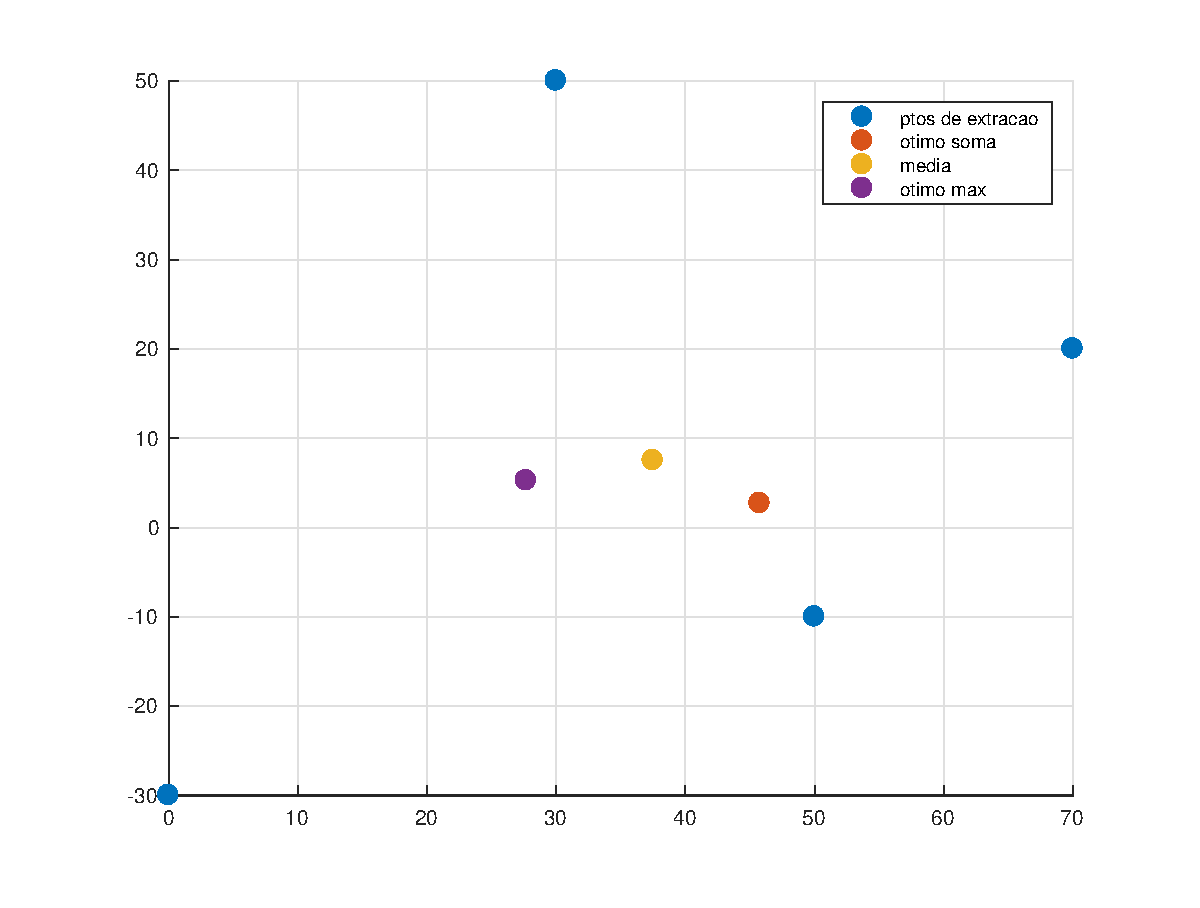
\includegraphics[width=10cm]{C2P20.eps}
    \captionof{figure}{Soluções ótimas do Problema 2.20. O ponto amarelo corresponde à solução ótima utilizando quadrados mínimos.}
    \label{fig:2.20}
\end{center}
\end{solution}

% 2.21	 % % % % % % % % % % % % % % % % % % % % %
%\setcounter{question}{74}
\question{\textbf{Tamanho de Lote Ótimo}. Uma empresa de instrumentação vende seu produto principal a uma taxa de 5 equipamentos por dia. Este tipo de instrumento é produzido em lotes regularmente. A companha gasta R\$ 2\,000 para preparar a produção de um lote e R\$ 40 por unidade e por dia para armazená-la no seu estoque após produzida. A companhia deseja escolher o tamanho ótimo do lote a ser produzido para minimizar o custo diário esperado de estoque e de preparação para a produção; assuma que a demanda siga a taxa fielmente. Formule e resolva este problema de otimização em uma variável.
}
\begin{solution}
	Seja $r = 5$ a taxa de equipamentos vendidos por dia, $c_A = 40$ o custo por unidade e por dia para armazenar os equipamentos, $c_P$ o custo de produção do lote, $x$ o tamanho do lote, $T = x/r$ o tempo para acabar o lote, $E(t) = x-rt$ o tamanho do estoque no tempo $t\in[0,T]$ e $\bar m = \frac{1}{T}\int_T E(t)\mathrm{d}t$ o número médio de equipamentos no estoque. Então, o custo médio diário de produção é dado por
    \begin{align*}
    	\bar c 	&= \frac{c_P}{T} + c_A\,\bar m \\
        		&= \frac{c_P\,r}{x} + c_A \frac{1}{T}\int_0^T(x-rt)\mathrm{d}t \\
                &= \frac{c_P\,r}{x} + c_A (x-rT/2) \\
                &= \frac{c_P\,r}{x} + c_A (x-x/2) \\
                &= \frac{c_P\,r}{x} + \frac{c_A}{2}x.
    \end{align*}
    Logo, a função objetivo é dada por $f_0(x) = \frac{c_P\,r}{x} + \frac{c_A}{2}x$ e o problema de otimização é $\min_{x\in\Z_+} f_0(x)$. Porém, usando os inteiros positivos o problema fica complicado, então vamos relaxar o problema e utilizar os reais positivos, ou seja, nosso novo problema é $\min_{x\in\R_+} f_0(x)$. Podemos fazer isso, pois $\Z_+ \subset \R_+$. Usando a condição de otimalidade de primeira ordem, temos
    \begin{align*}
    		&\frac{\mathrm{d}f_0}{\mathrm{d}x}(x^*) = 0 \\
        \Rightarrow~ &\frac{c_A}{2} - \frac{c_P\,r}{{x^*}^2} = 0 \\
        \Rightarrow~ &\boxed{x^* = \sqrt{2r\frac{c_P}{c_A}} = 10\sqrt{5}}.
    \end{align*}
    A solução encontrada é ótimo global no problema relaxado, pois a função objetivo é convexa ${f_0''(x) > 0}~{\forall x\in\R_+}$. Porém, lembremos que o problema original está nos inteiros, então testamos o inteiro inferior $\lfloor x^*\rfloor = 22$ e o superior $\lceil x^*\rceil = 23$ mais próximos. Como $f_0(\lfloor x^*\rfloor)<f_0(\lceil x^*\rceil)$, a solução é 22 para o número ótimo de lote.
\end{solution}

\end{questions}

\newpage

% \setcounter{section}{4}
% \section{Exercícios Teóricos}
% \begin{questions}

% 5.27 % % % % % % % % % % % % % % % % % % % % %
\setcounter{question}{26}
\question{
Se $X$ é uniformemente distribuída em $(a, b)$, qual variável aleatória que varia linearmente com $X$ é uniformemente distribuída em $(0, 1)$?
}
\begin{solution}
Seja $Y = (X-a)/(b-a)$, então
\begin{align*}
	F_Y(y) &= P(Y\le y) = P((X-a)/(b-a) \le y)\\
    	&= P(X \le (b-a)\,y+a) = F_X((b-a)\,y+a).
\end{align*}
Derivando os dois lados da equação em relação à $y$ obtemos que
\begin{align*}
	f_Y(y) =  (b-a)f_X((b-a)\,y+a) =
    \begin{cases}
    	1, &\text{se }y\in(0,1);\\
        0, &\text{caso contrário.}
    \end{cases}
\end{align*}
Logo, $Y$ é uniformemente distribuída em $(0,1)$.\\[1mm]
\textit{Observação:} outra opção é fazer $Y = (b-X)/(b-a)$.
\end{solution}

% 5.29 % % % % % % % % % % % % % % % % % % % % %
\setcounter{question}{28}
\question{
Seja $X$ uma variável aleatória contínua
com função distribuição cumulativa $F$.
Defina a variável aleatória $Y$ como $Y = F(X)$.
Mostre que $Y$ é uniformemente distribuída em $(0, 1)$.
}
\begin{solution}
	Por simplicidade, vamos supor que $F: \mathbb{R} \to [0,1]$ seja estritamente crescente. Logo, $F$ é inversível e para $y \in (0,1)$,
	\begin{align*}
		F_Y(y) = P(Y\le y) = P(F(X)\le y) = P(X \le F^{-1}(y)) = F(F^{-1}(y)) = y.
	\end{align*}
    Dessa forma, quando $y \in \mathbb{R}$,
    \begin{align*}
    	F_Y(y) =
        \begin{cases}
    	0, &\text{se }y \le 0;\\
        y, &\text{se }0 < y < 1;\\
        1, &\text{se }y \ge 1;\\
    	\end{cases}
    \end{align*}
    o que caracteriza uma distribuição uniforme em $(0,1)$.\\[1mm]
    \textit{Observação:} Isso também acontece quando $F$ não é inversível.
\end{solution}

% 5.30 % % % % % % % % % % % % % % % % % % % % %
%\setcounter{question}{28}
\question{
Suponha que $X$ tenha função densidade
de probabilidade $f_X$. Determine a função
densidade de probabilidade da variável
aleatória $Y$ definida como $Y = aX + b$.
}
\begin{solution}
	Seja $a>0$,
	\begin{align*}
		F_Y(y) = P(Y\le y) = P(aX+b\le y) = P(X\le (y-b)/a) = F_X((y-b)/a).
	\end{align*}
    Derivando ambos lados da equação em relação à $y$ leva à
    \begin{align*}
    	f_Y(y) = \frac{f_X((y-b)/a)}{a}.
    \end{align*}
    Por outro lado, se $a<0$, então
    \begin{align*}
    	F_Y(y) &= P(X\ge (y-b)/a) = 1-P(X<(y-b)/a) = 1-F_X([(y-b)/a]^-)\\
        	&= 1-F_X((y-b)/a) \quad\text{(a variável aleatória é contínua).}
    \end{align*}
    Novamente, derivando ambos lados da equação em relação à $y$ leva à
    \begin{align*}
    	f_Y(y) = \frac{f_X((y-b)/a)}{-a}.
    \end{align*}
    Portanto, quando $a\neq 0$,
    \begin{align*}
    	f_Y(y) = \frac{f_X((y-b)/a)}{|a|}.
    \end{align*}
\end{solution}

\end{questions}
%\newpage

% \vspace{10mm} {\LARGE \textbf{Desafio!}}
% \begin{enumerate}
% \item Um investidor comprou uma ação muito instável. A cada mês, o valor dessa ação segue uma distribuição uniforme no intervalo $(0,1000)$ e é independente dos meses anteriores. O investidor pode vender a ação quando quiser, porém a cada mês que passa o dinheiro, para o investidor, vale $d$ vezes o mês anterior ($0<d<1$). Qual estratégia ele deve seguir para maximizar o retorno esperado na venda dessa ação? Se $d=4/5$, qual deve ter sido o valor máximo pago na compra da ação para que o investidor tenha um valor esperado de lucro positivo?
% \end{enumerate}

\end{document}